
\chapter{Export your map}

\pagestyle{fancy}
\fancyhf{}
\fancyhead[OC]{\leftmark}
\fancyhead[EC]{\rightmark}
%\renewcommand{\footrulewidth}{1pt}
\cfoot{\thepage}

%%%%%%%%%%%%%%%%%%%%%%%%%%%%%%%%%%%%%%%%%%%%%%%%%%%%%%%%%%%
%%%%%%%%%%%%%%%%%%%%%%%%%%%%%%%%%%%%%%%%%%%%%%%%%%%%%%%%%%%

To get the maps out of the software and into your report, apart from using Snipping tool/shutter, QGIS offers two options.

\section{To save just the contents of the map canvas: Export}
Project $\rightarrow$ Import/Export $\rightarrow$ Export map to pdf.\\
Project $\rightarrow$ Import/Export $\rightarrow$ Export map to image.

\section{To save items in addition to the map canvas: Print layout}
Compose a sheet with multiple items, such as the map, legend, titles, tables etc.\\

Project $\rightarrow$ New Print Layout.


\begin{figure}[!h]
	\centering
	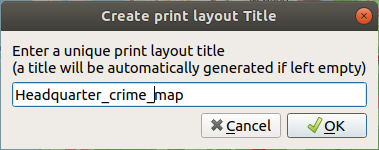
\includegraphics[width=0.25\textwidth]{images/create_print_layout_name.png}
	\caption{Enter the title of your layout. This title will appear under Project $\rightarrow$ Layouts}
	\label{ft_fig_firstfig3}
\end{figure}

Print layout has it's own window, menu, tools and panels.\\
Once a layout has been created, can close the layout window and reopen it under Project $\rightarrow$ Layouts. The title you give the layout is what will appear in the “Layouts” list.\\

To change the orientation between Landscape \& Portrait, right click on the page in the layout and select page properties. This will add the “item properties” tab on the RHS of the window


\begin{figure}[!h]
	\centering
	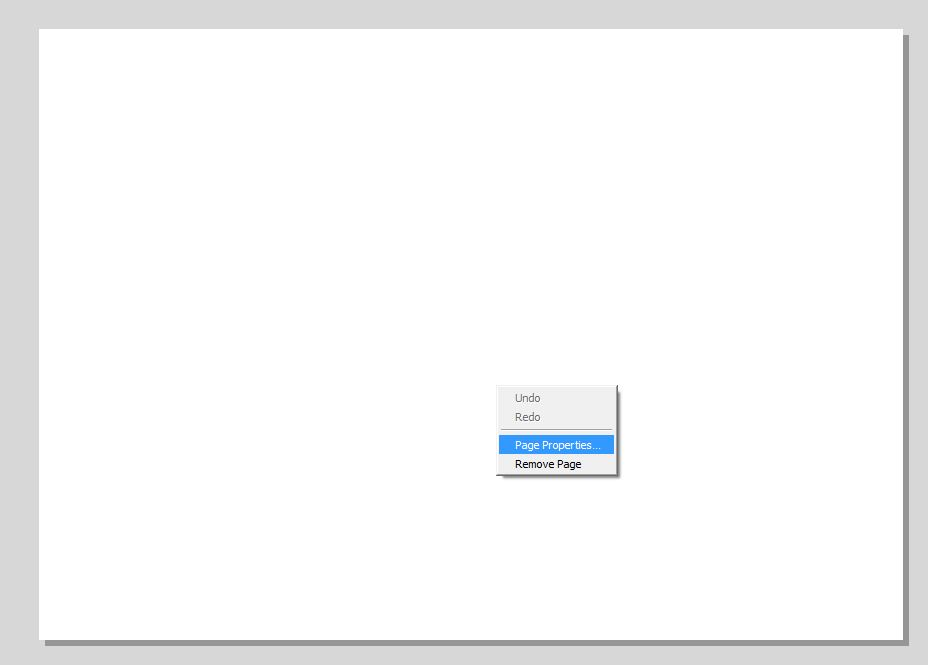
\includegraphics[width=0.4\textwidth]{images/print_layout_orientation.png}
	\caption{To change page orientation}
	\label{ft_fig_firstfig3}
\end{figure}

\begin{figure}[!h]
	\centering
	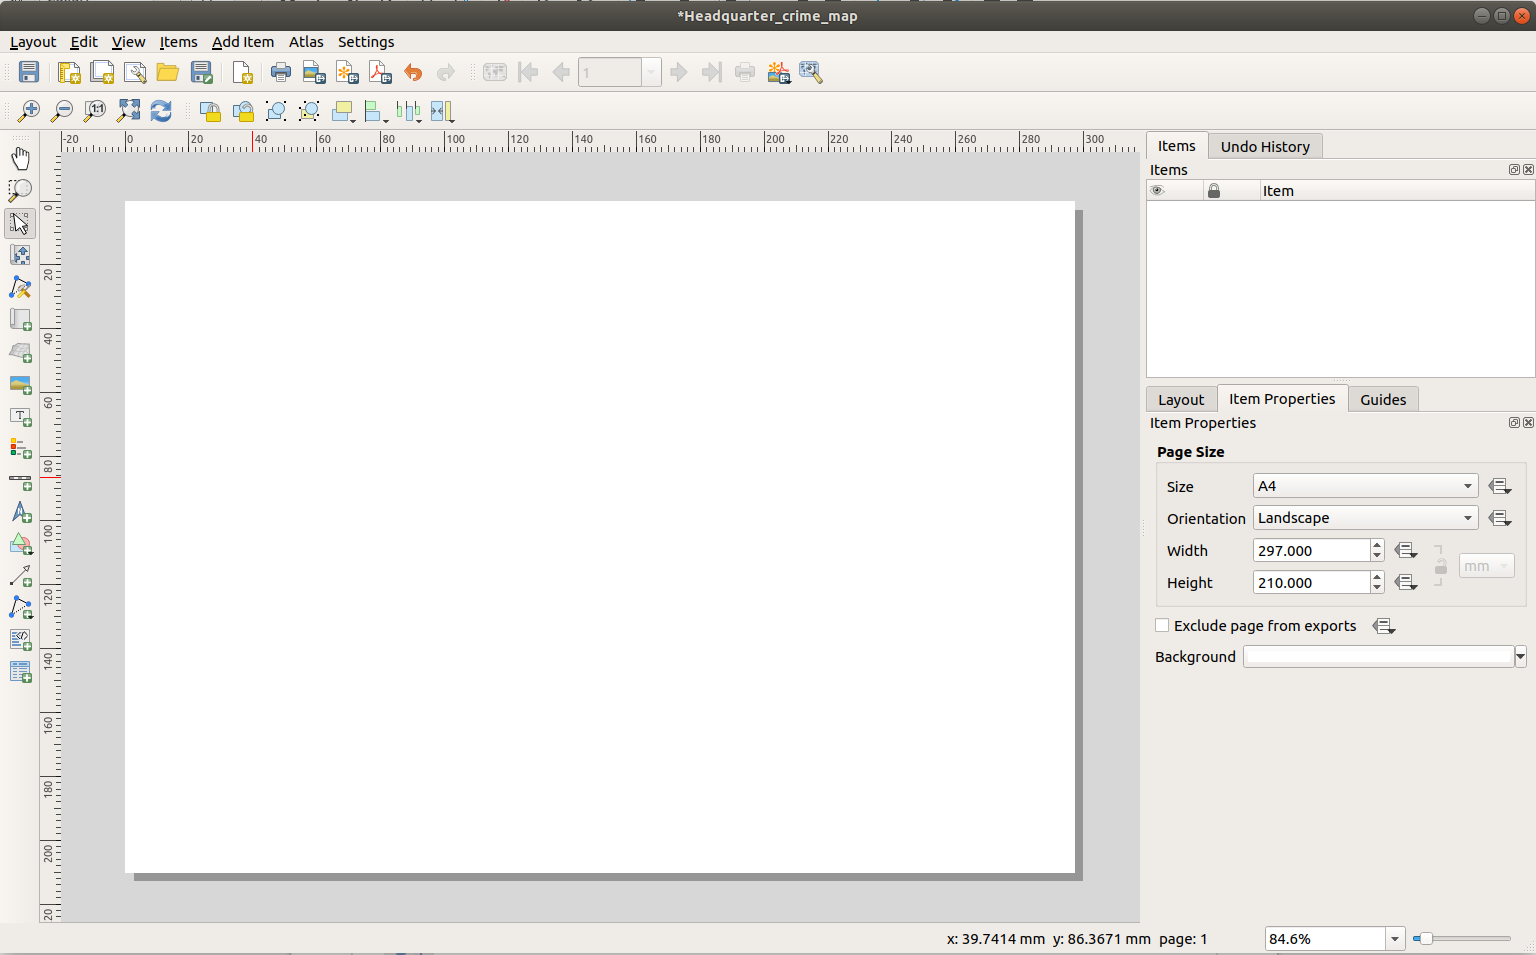
\includegraphics[width=0.7\textwidth]{images/print_layout_full_window.png}
	\caption{Layout window. Main tools on LHS toolbar}
	\label{ft_fig_firstfig3}
\end{figure}

The main items that you will add to your layout are found in the LHS toolbar. Each item on the layout will be added to the list in the Items panel. To edit an item either select it on the layout, or highlight it from the items list.\\
\begin{tabular}{@{}c@{}}
\includegraphics[width=4ex]{images/adds_a_new_map_to_the_layout_icon.png}\end{tabular} Adds a new Map to the layout: will bring the map canvas from QGIS that you have just been working on.

\begin{tabular}{@{}c@{}}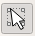
\includegraphics[width=4ex]{images/select_move_item_icon.png}\end{tabular}
  Select/move item.  So can grab an item on the layout and move it, resize it

\begin{tabular}{@{}c@{}}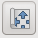
\includegraphics[width=4ex]{images/move_item_content_icon.png}\end{tabular}
Move item content.  So can reposition the map content within the window.  It’s like panning about within the QGIS map canvas been doing previously


\begin{tabular}{@{}c@{}}
\includegraphics[width=4ex]{images/refresh_icon.png}\end{tabular}
Refresh.  If you have revisited the map in QGIS and made changes, may need to give the layout a nudge to update.

\begin{tabular}{@{}c@{}}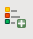
\includegraphics[width=4ex]{images/add_legend_icon.png}\end{tabular}
Add legend.  As default all the layers are included in the legend. Customise which layers are included in the legend in the items panel on the RHS, untick Auto Update (under the Legend Items title).  
Use + \& - buttons to have the items want.  Edit the text in the print layout (double click)
Size of the text does not scale automatically as resize the legend window. Instead edit each component size (text) and symbols (the colours).

\begin{tabular}{@{}c@{}}
\includegraphics[width=4ex]{images/add_new_label_icon.png}\end{tabular}
Add a new label: give your map a title


\begin{tabular}{@{}c@{}}
\includegraphics[width=4ex]{images/add_attribute_table_icon.png}\end{tabular}
Add attribute table.  Choose the columns to include, the max number of rows to include, can filter the rows that can be included based on a column value…

\begin{tabular}{@{}c@{}}
\includegraphics[width=4ex]{images/add_arrow_icon.png}\end{tabular}
Add arrow

\begin{tabular}{@{}c@{}}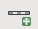
\includegraphics[width=4ex]{images/add_scale_bars_icon.png}\end{tabular}
Add scale bars\\
Item properties $\rightarrow$ Segments $\rightarrow$ Left 2\\
Item properties $\rightarrow$ Segments $\rightarrow$ Right 4

\begin{tabular}{@{}c@{}}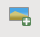
\includegraphics[width=4ex]{images/add_image_icon.png}\end{tabular}
Add image (chose image file from computer)\\

In the top toolbar find the useful undo and redo buttons \begin{tabular}{@{}c@{}}
\includegraphics[width=4ex]{images/undo_redo_layout_icons.png}\end{tabular}\\


Following the copyright and licencing rules if using OpenStreetMap \url{https://www.openstreetmap.org/copyright}, add a label to contain the information \textbf{${\textcopyright}$ OpenStreetMap contributors, licenced as CC BY-SA}, and it is also good practice to acknowledge the software, \textbf{Created in QGIS}.\\


Export this map.  Select: Layout $\rightarrow$ Export as image. Select location, file name and file type (PNG ~7MB)

%\begin{figure}[!h]
%	\centering
%	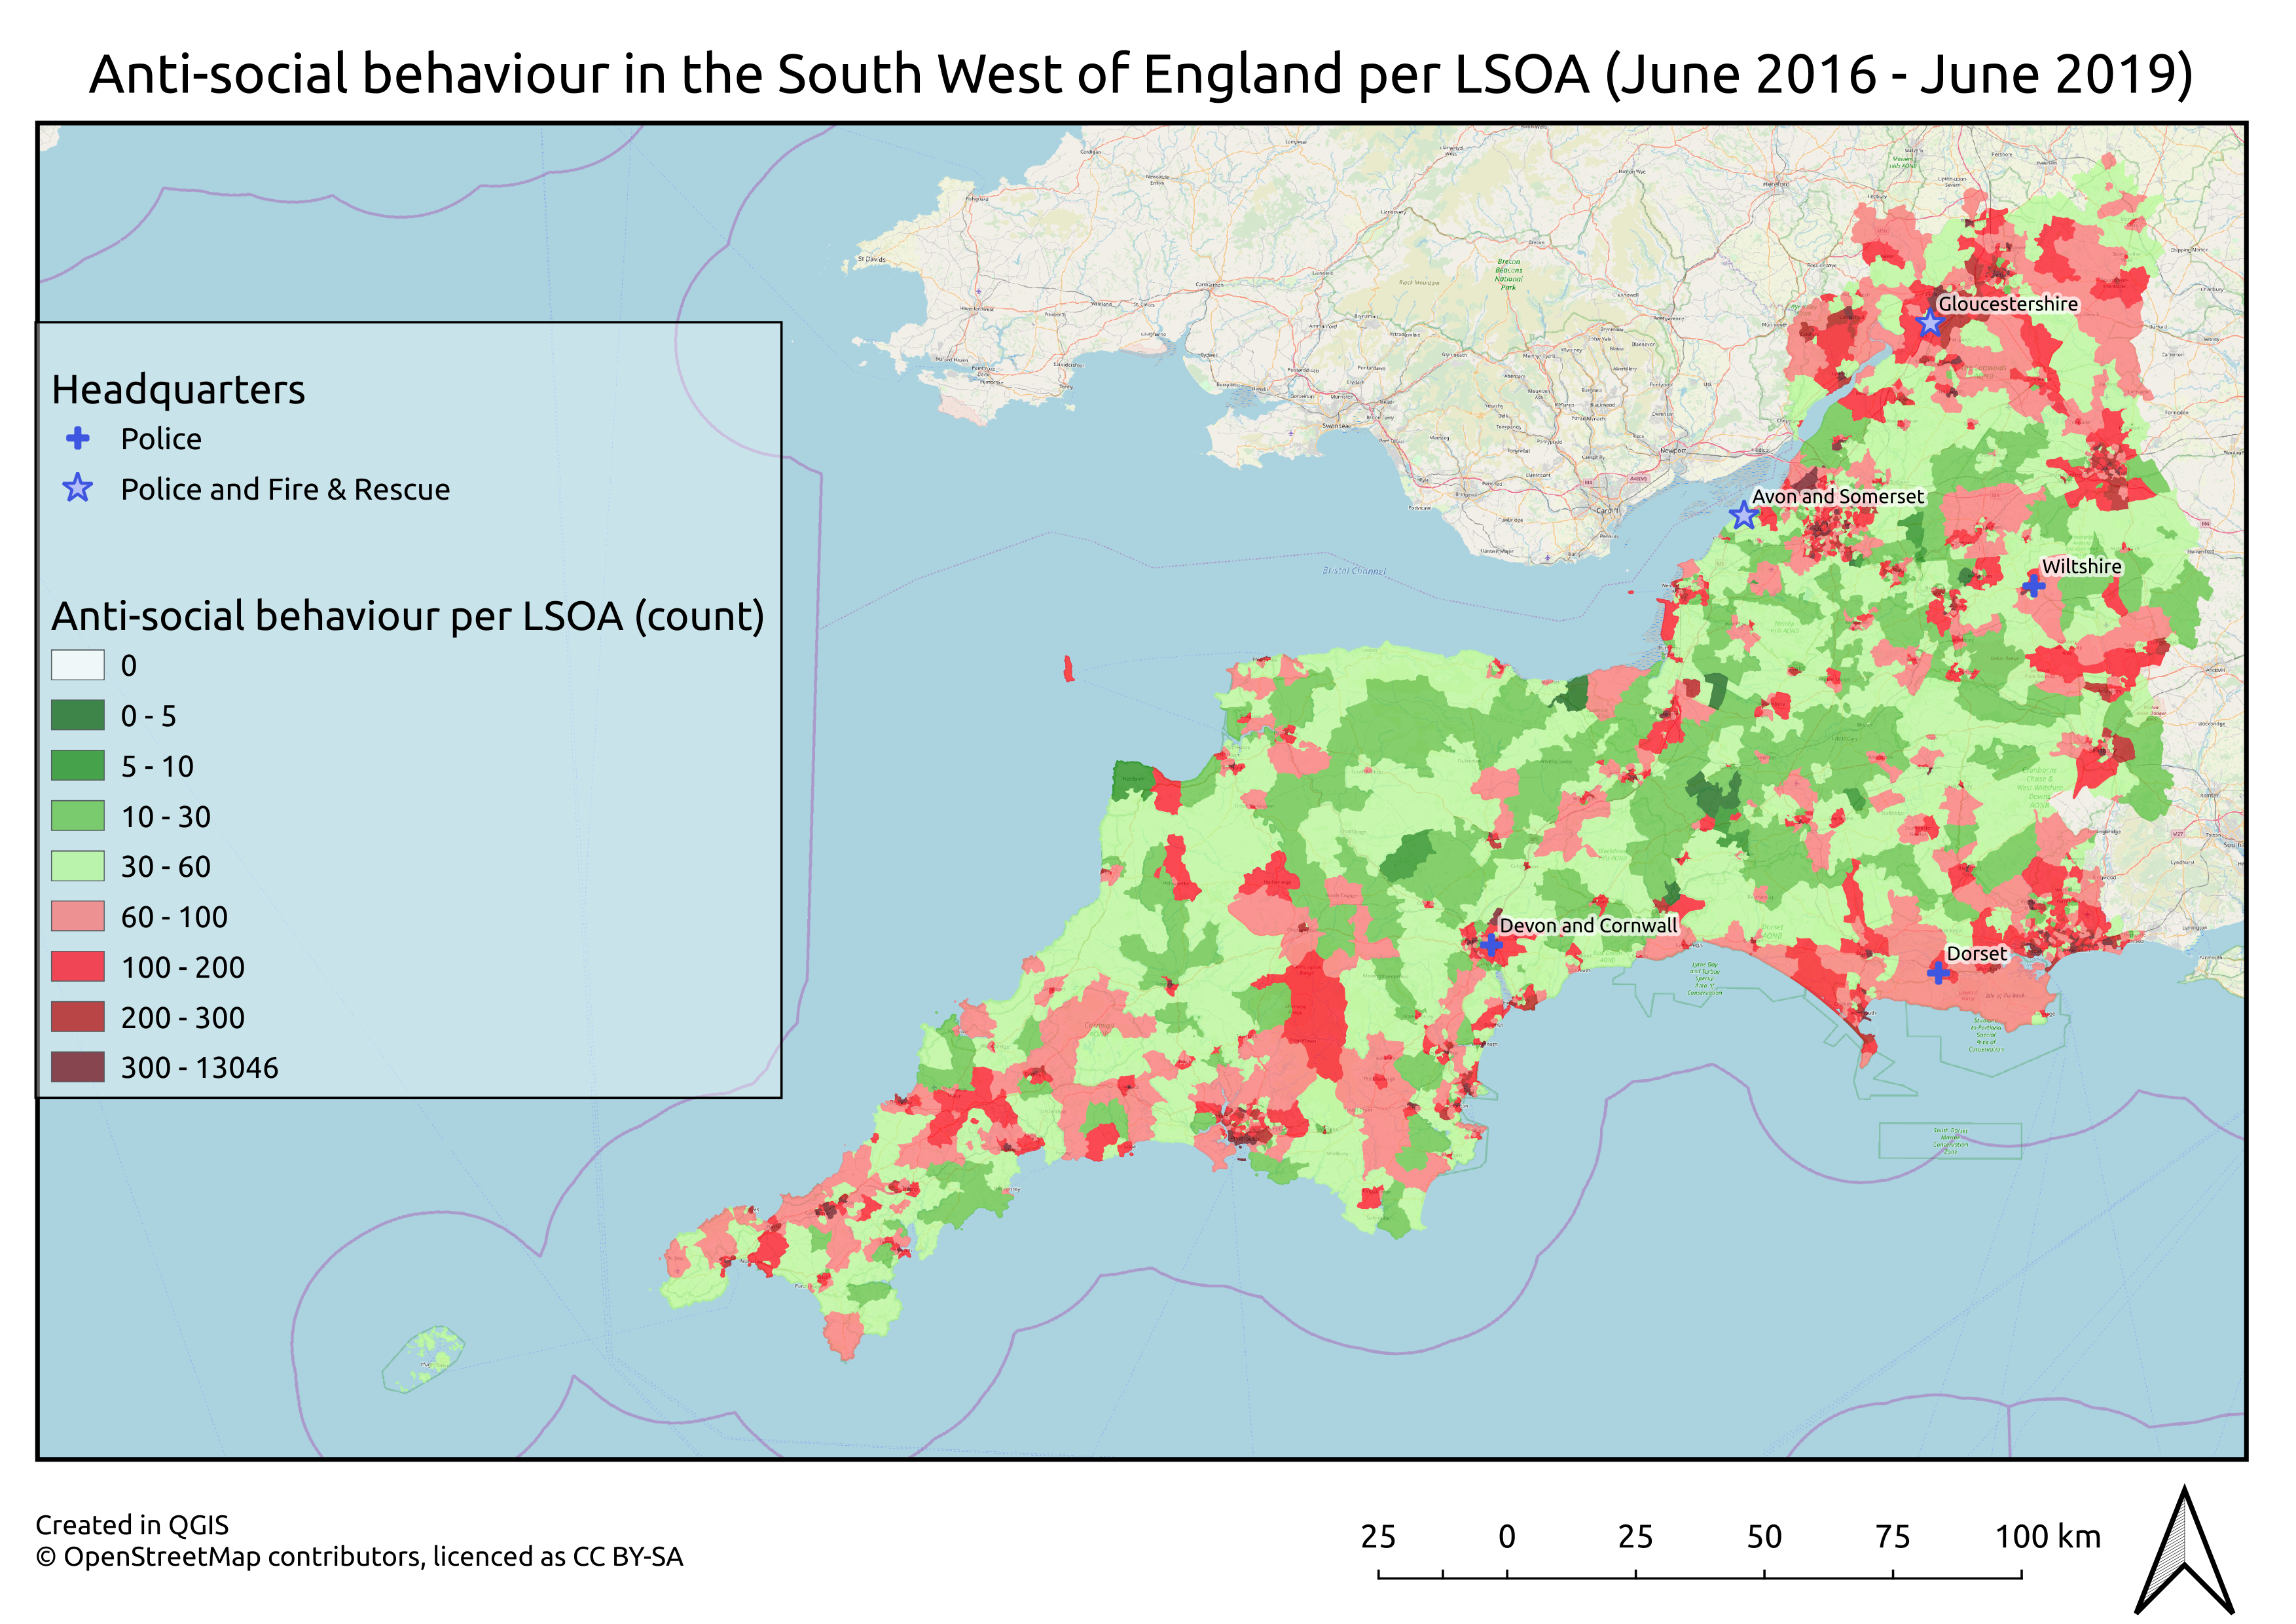
\includegraphics[width=0.9\textwidth]{images/headquarter_crime_map.png}
%	\caption{}
%	\label{ft_fig_firstfig3}
%\end{figure}


